\documentclass[12pt]{article}
\usepackage[utf8]{inputenc}
\usepackage[english]{babel}
\usepackage{float}
\usepackage{pythonhighlight}
\usepackage{graphicx}

\renewcommand{\baselinestretch}{1.3}

\usepackage{biblatex}
\addbibresource{cw2.bib}


\newcommand{\numpy}{{\tt numpy}}    % tt font for numpy

\topmargin -.5in
\textheight 9in
\oddsidemargin -.25in
\evensidemargin -.25in
\textwidth 7in

\begin{document}

% ========== Edit your name here
\author{Baran Buluttekin\\13153116}
\title{Data Science Techniques and Applications\\Coursework II}
\date{March 23, 2019}
\maketitle

\medskip

\indent We can start of our analysis by getting the dataset. Corresponding Heart Diseases dataset\cite{kaggle}\cite{uci-source} can be downloaded from kaggle by clicking download link in the website. When the download finished we received compressed version of file named \textit{heart-disese-uci.zip}. Fallowing the un-compression of the file we will obtain csv file \textit{heart.csv} which is in final format for analysis. 

Next step is to loading python libraries to start the analysis. In this coursework fallowing open source libraries used:
\begin{enumerate}
    \item \textbf{Pandas: }Tabular data manipulation library that will be use to load the data and cleaninig/reshaping.\cite{mckinney-proc-scipy-2010}
    \item \textbf{Matplotlib: }Will be used as main plotting library that has many pre build high level plotting tools.\cite{matplotlib}
    \item \textbf{Seaborn: }Python library for special plotting styles such as pairplots.\cite{seaborn}
    \item \textbf{Scikit-Learn: }Open source machine learning library that includes various machine learning algorithms.\cite{scikit-learn}
\end{enumerate}

As a first step libraries above loaded in python in the fallowing format.

\begin{python}
    import pandas as pd
    import matplotlib.pyplot as plt
    from mpl_toolkits.mplot3d import Axes3D
    from sklearn.decomposition import PCA
    import seaborn as sns
\end{python}

With the help of pandas library we can load the dataset and view first 5 rows to check if the data frame is in expected format.

\begin{python}
    df = pd.read_csv("heart.csv")
    df.head()
\end{python}

\begin{table}[h!]
    \centering
     \begin{tabular}{||c c c c c c c c c c c c c c||} 
     \hline
     age & sex & cp & trestbps & chol & fbs &restecg & thalach & exang & oldpeak & slope & ca & thal & target \\ [0.5ex] 
     \hline\hline
     63.0 & 1.0 & 3.0 & 145.0 & 233.0 & 1.0 & 0.0 & 150.0 & 0.0 & 2.3 & 0.0 & 0.0 & 1.0 & 1.0\\ 
     37.0 & 1.0 & 2.0 & 130.0 & 250.0 & 0.0 & 1.0 & 187.0 & 0.0 & 3.5 & 0.0 & 0.0 & 2.0 & 1.0\\
     41.0 & 0.0 & 1.0 & 130.0 & 204.0 & 0.0 & 0.0 & 172.0 & 0.0 & 1.4 & 2.0 & 0.0 & 2.0 & 1.0\\
     56.0 & 1.0 & 1.0 & 120.0 & 236.0 & 0.0 & 1.0 & 178.0 & 0.0 & 0.8 & 2.0 & 0.0 & 2.0 & 1.0\\
     57.0 & 0.0 & 0.0 & 120.0 & 354.0 & 0.0 & 1.0 & 163.0 & 1.0 & 0.6 & 2.0 & 0.0 & 2.0 & 1.0\\ [1ex] 
     \hline
     \end{tabular}
    \end{table}

Fallowing the guide of coursework, I choose "age", "chol" and "trestbps" as important dimensions. Description of the columns from the coursework I is given below as a reminder.

\begin{quote}
    \begin{enumerate}
        \item \textbf{age}: Age in years (max:77, min:29)
        \item \textbf{chol}: cholesterol level (mg/dl)
        \item \textbf{trestbps}: Blood pressure recording for resting
    \end{enumerate}
\end{quote}

In order to get a better grasp of the data distribution with these three variables, I will use pairplot. Pairplot will help us see different variation of these three variable with each other and with relation to the target outcome of the dataset.

\begin{python}
    selected_dims = ["age", "chol", "trestbps", "target"]
    sns.pairplot(df[selected_dims], hue="target")
\end{python}

\begin{figure}[H]
    \centering
    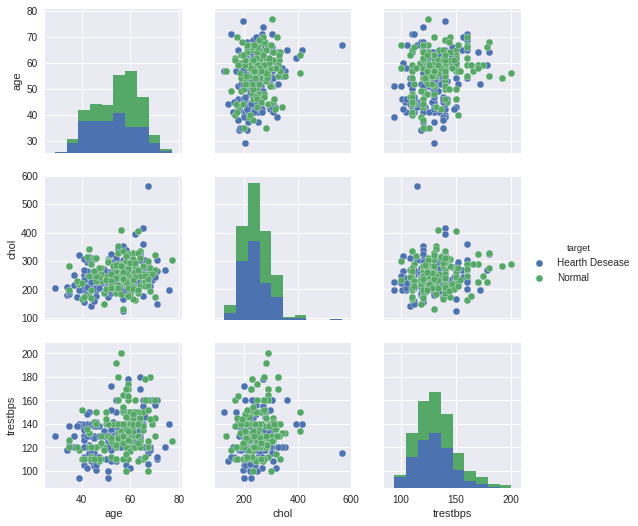
\includegraphics[width=\textwidth]{img/pairplot.png}
    \caption{Pairplot with chosen dimensions.}
\end{figure}
 
We can also plot these 3 dimensions in 3D plot to see their relation to target variable. I created helper function quickly plot 3D plots given dimensions in dataset. Code for the function follows.

\begin{python}
    def plot_3d(dataframe, x_label, y_label, z_label, target_label, title):
        labelTups = [("Normal", 0), ("Hearth Desease", 1)]
        fig = plt.figure(1, figsize=(8, 6))
        ax = Axes3D(fig, elev=-150, azim=110)
        ax.scatter(dataframe[x_label], dataframe[y_label], dataframe[z_label], c=dataframe[target_label],
                    cmap=plt.cm.Set1, edgecolor='k', s=40)
        ax.set_title(title)
        ax.set_xlabel(x_label)
        ax.w_xaxis.set_ticklabels([])
        ax.set_ylabel(y_label)
        ax.w_yaxis.set_ticklabels([])
        ax.set_zlabel(z_label)
        ax.w_zaxis.set_ticklabels([])

        sc = ax.scatter(dataframe[x_label], dataframe[y_label], dataframe[z_label], c=dataframe[target_label], cmap="Spectral", edgecolor='k')

        colors = [sc.cmap(sc.norm(i)) for i in [1, 0]]
        custom_lines = [plt.Line2D([],[], ls="", marker='.', 
                        mec='k', mfc=c, mew=.1, ms=20) for c in colors]
        lgd = ax.legend(custom_lines, [lt[0] for lt in labelTups], 
                    loc='center left', bbox_to_anchor=(1.0, .5))
        plt.show()
\end{python}

We can observe their relationships by calling the function with the \textit{"age"}, \textit{"chol"} and \textit{"trestbps"}.

\begin{python}
    plot_3d(df, "age", "chol", "trestbps", "target", "Heart Desease clustering by 3 dimensions")
\end{python}

\begin{figure}[H]
    \centering
    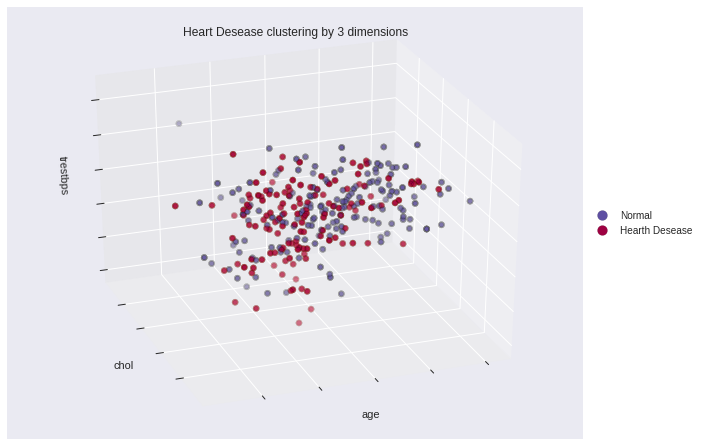
\includegraphics[width=\textwidth]{img/3d-selected.png}
    \caption{3D graph of the selected dimensions.}
\end{figure}

\section*{Applying PCA On Dataset}



\printbibliography
\end{document}